\chapter{Límites de uso y \textit{rates}}
\label{cap:limites}

Este capítulo responde a la RQ3: cómo se relacionan los límites de uso y los \textit{rates} en las APIs de correo, y qué implicaciones tiene esa relación para el consumidor.
Un límite de uso es el máximo de un nivel de uso medible, como los correos enviados al mes o los días que se conservan los registros, y puede renovarse o no.
La cuota es un límite de uso renovable: el volumen máximo que se puede enviar en un periodo, llamado ventana, y que se repone cuando la ventana se cierra.
El \textit{rate}, o caudal, es la velocidad máxima de envío, en peticiones o en correos por unidad de tiempo.

En seis de las ocho APIs, si la cuenta no está en revisión, en pruebas ni restringida por reputación, al ritmo máximo del \textit{rate} la cuota se agota antes de que acabe su ventana, así que lo que frena el envío es la cuota.
En las otras dos no se puede decir lo mismo: Amazon SES no publica la cuota ni el \textit{rate} de su cuenta de producción, y en la cuenta de prueba de Mailchimp Transactional el caudal, de 25 correos por hora, frena antes que la cuota.

El capítulo se organiza del siguiente modo.
En primer lugar, la Sección~\ref{sec:limites:geometrica} define las cuatro magnitudes del cálculo (el \textit{rate}, la cuota, su ventana y los destinatarios por petición) y la curva de capacidad que las combina.
A continuación, la Sección~\ref{sec:limites:publicado} recoge lo que publica cada proveedor y calcula, plan a plan, cuántas veces cabe la cuota en lo que el \textit{rate} admite durante su ventana.
Después, la Sección~\ref{sec:limites:catalogo} extrae seis afirmaciones con su recuento sobre las ocho APIs, y la Sección~\ref{sec:limites:prime4api} contrasta el cálculo a mano con las respuestas de PRIME4API.
Por último, la Sección~\ref{sec:limites:respuesta} responde a la RQ3.

\section{Lectura geométrica}
\label{sec:limites:geometrica}
\label{sec:hallazgos:limites-rates}

En el plan Pro de Resend el \textit{rate} es de 10 peticiones por segundo, el valor por defecto que el proveedor publica por equipo, compartido por todas sus claves de API \citep{resenddocs}.
A ese ritmo, un mes de 30 días admite 25.920.000 peticiones, y la cuota del plan es de 50.000 correos al mes \citep{resendpricing}.
Al ritmo máximo, en esos 30 días cabría, por tanto, 518 veces la cuota, contando un destinatario por petición.
En SendGrid Essentials 50K \citep{sendgridpricing} el mismo cálculo da 518.400 veces, con un \textit{rate} de 10.000 peticiones por segundo.
El proveedor publica ese \textit{rate} una sola vez, en una pregunta frecuente que no lo liga a ningún plan.
En la cuenta de prueba de Mailchimp Transactional el cálculo no se puede hacer.
Su franquicia de 500 correos no tiene ventana declarada, y lo único que pone tiempo es un caudal de 25 correos a la hora \citep{mailchimpdocs}.

El cálculo usa cuatro magnitudes de la Datasheet.
El \textit{rate} $R$ se expresa en peticiones por segundo y sale del bloque \texttt{max\_power}.
La cuota $Q$ se expresa en correos, y su ventana $W$, el periodo tras el que la cuota se repone (un día o un mes), en segundos.
Las dos están en el bloque \texttt{capacity}.
El factor $k$ es el número de destinatarios que lleva cada petición, de uno al máximo que admite el proveedor, que la Datasheet declara en el bloque \texttt{workload}.

El factor $k$ corresponde al «CRF» (\textit{Consumption Request Factor}) de Gavira Sánchez \citep{gavira2026tfm}, la regla que dice cuántas unidades de una métrica descuenta cada petición.
Contar $k$ en destinatarios supone que cada destinatario descuenta una unidad de cuota.
Esa equivalencia está sostenida en cuatro de las ocho APIs: Resend y SendGrid la publican, y en Brevo y Amazon SES la midió un sondeo, una tanda de peticiones reales contra la API para medir un límite (Apartado~\ref{sec:propuesta:validacion}).
En Postmark, MailerSend, Mailgun y Mailchimp no consta que cada destinatario descuente una unidad de cuota.

Para un envío uniforme a un ritmo medio $c$, en correos por segundo, los dos límites fijan dos umbrales de ritmo y un tiempo:
\begin{equation}
c_{\mathrm{cuota}} = \frac{Q}{W}, \qquad c_{\mathit{rate}} = R \cdot k, \qquad t_{\min} = \frac{Q}{R \cdot k}.
\label{eq:limites-rates}
\end{equation}
El primer umbral es el ritmo medio que agota la cuota justo al cerrar su ventana.
El segundo es el ritmo máximo de correos que admite el \textit{rate}.
El tiempo $t_{\min}$ es el que tarda una ráfaga sostenida a ese ritmo máximo en agotar la cuota.

De los dos límites, la restricción activa es el de umbral menor: el que se alcanza primero y frena el envío, mientras el otro no llega a actuar.
En Resend Pro la cuota pide 0,019 correos por segundo de media y el \textit{rate} admite 10, así que la restricción activa es la cuota.
El cociente $R \cdot W / Q$ compara los dos topes en la misma ventana: cuántas veces cabría la cuota en lo que el \textit{rate} admite en ella: 518 en Resend Pro y 518.400 en SendGrid Essentials 50K.
Se calcula con $k = 1$ para comparar las APIs en peticiones, y $k$ solo entra en el umbral del \textit{rate} y en $t_{\min}$.

Las cuatro magnitudes son las que PRIME4API lee de la Datasheet para construir los límites de cada plan \citep{gavira2026tfm}.
El mes se toma de 30 días (2.592.000 segundos) y el día de 86.400 segundos.
Con meses de 31 días los cocientes cambian un 3,3~\%.

Con ocho APIs, esta notación no cubre tres casos: los dos contadores de Mailgun, el caudal de Mailchimp en correos por hora y su franquicia sin ventana.
En Mailgun, la cabecera de la respuesta de cada envío aceptado trae dos contadores sobre el mismo \textit{endpoint}: uno de 80.000 peticiones y otro de 2.000.000 de destinatarios.
Los dos comparten una ventana que Mailgun no publica y que dos mediciones situaron en unos diez segundos (Sección~\ref{sec:limites:publicado}).
Hay entonces dos términos de \textit{rate}, $R$ en peticiones y $R_d$ en destinatarios, y cuál de los dos corta antes depende de $k$.
La Tabla~\ref{tab:limites-rates-b} calcula el cociente de Mailgun con el contador de peticiones, y el de destinatarios solo entra en su $t_{\min}$ con el $k$ máximo.

En Mailchimp el caudal se declara en correos por hora y no en peticiones, así que $k$ no multiplica nada: el \textit{rate} solo frena el envío cuando el ritmo medio supera los 25 correos por hora.
La franquicia de 500 correos de su cuenta de prueba tampoco tiene ventana.
Sin $W$ no hay cociente que formar, porque los 500 correos de la franquicia se gastan una sola vez y no se reponen.
En Mailchimp no se calcula el cociente y se anota el tipo de límite.

La misma relación se lee como una curva.
Ruiz-Cortés y Ruiz-López interpretan el \textit{rate} como la velocidad máxima de consumo y la cuota como el volumen máximo acumulable en un periodo, y la capacidad efectiva sale de aplicar los dos límites a la vez \citep{ruizcortes2025cajanegra}.
El ACM adopta esa interpretación como su semántica.
Sobre ella, la curva de capacidad $C(t)$ de Gavira Sánchez \citep{gavira2026tfm} es el máximo de correos acumulables desde el inicio de la ventana hasta el instante $t$ sin violar ningún límite.

Con un \textit{rate} y una cuota, la curva tiene dos tramos.
Mientras manda el \textit{rate}, la curva es una recta de pendiente $R \cdot k$.
Cuando manda la cuota, se vuelve horizontal a la altura de $Q$.
El codo entre ambos cae en $t_{\min}$.
Cuanto antes llega el codo dentro de la ventana, más holgado es el \textit{rate}.
Esa holgura se mide con $W / t_{\min} = R \cdot W \cdot k / Q$, que es el cociente $R \cdot W / Q$ multiplicado por $k$.
En Resend Pro con $k = 1$ el codo llega a los 5.000 segundos, unos 83 minutos, y el tramo horizontal ocupa el resto de los 30 días.
Con los 50 destinatarios por petición que admite Resend, el codo se adelanta a los 100 segundos.
La curva no recoge los dos contadores de Mailgun ni la franquicia sin ventana de Mailchimp.

\begin{figure}[H]
\centering
\subfigure[Resend Pro, $k = 1$ (3 horas)]{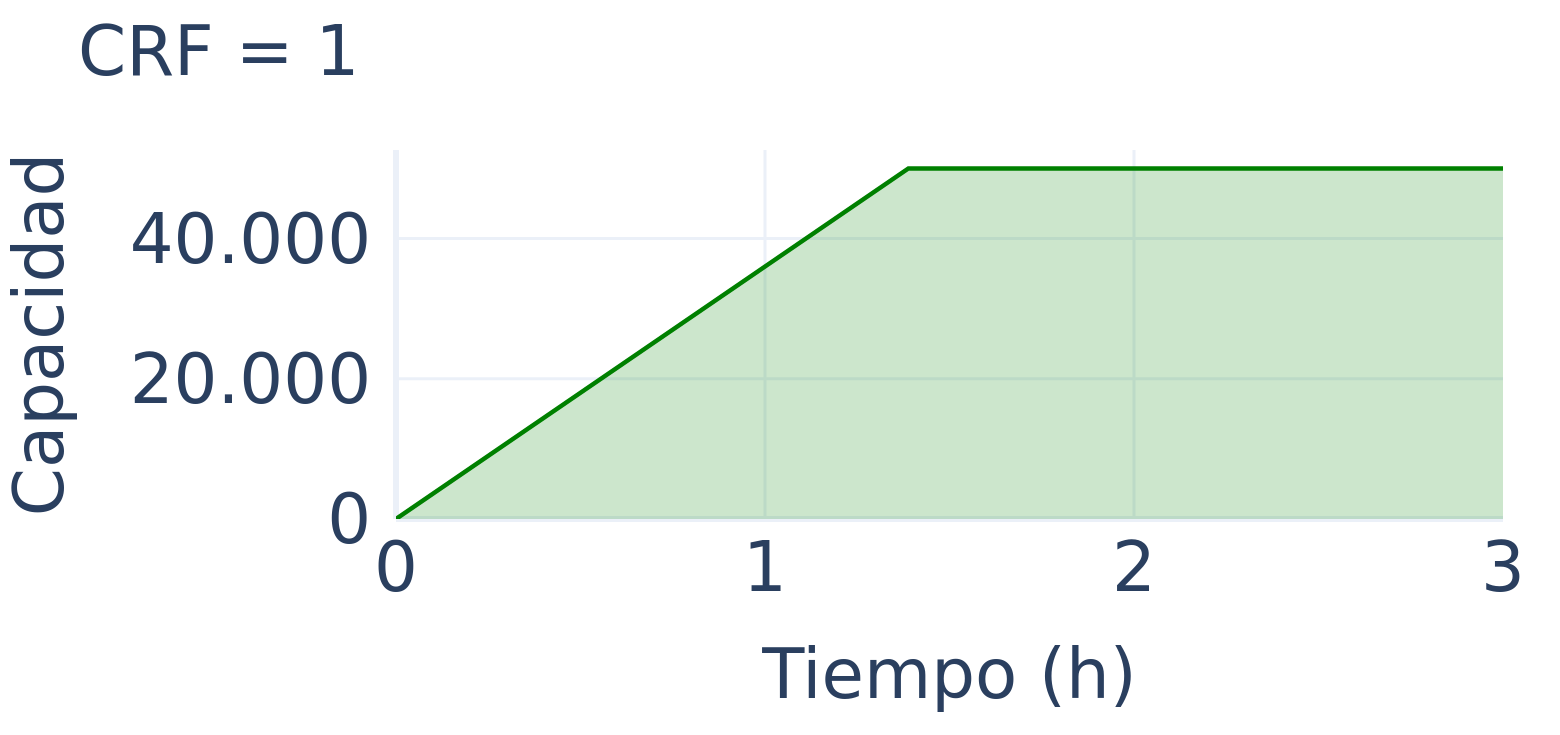
\includegraphics[width=0.42\textwidth]{fig/capacidad_resend_pro_k1_2026-10-25.png}}
\subfigure[SendGrid Essentials 50K, $k = 1.000$ (5 segundos)]{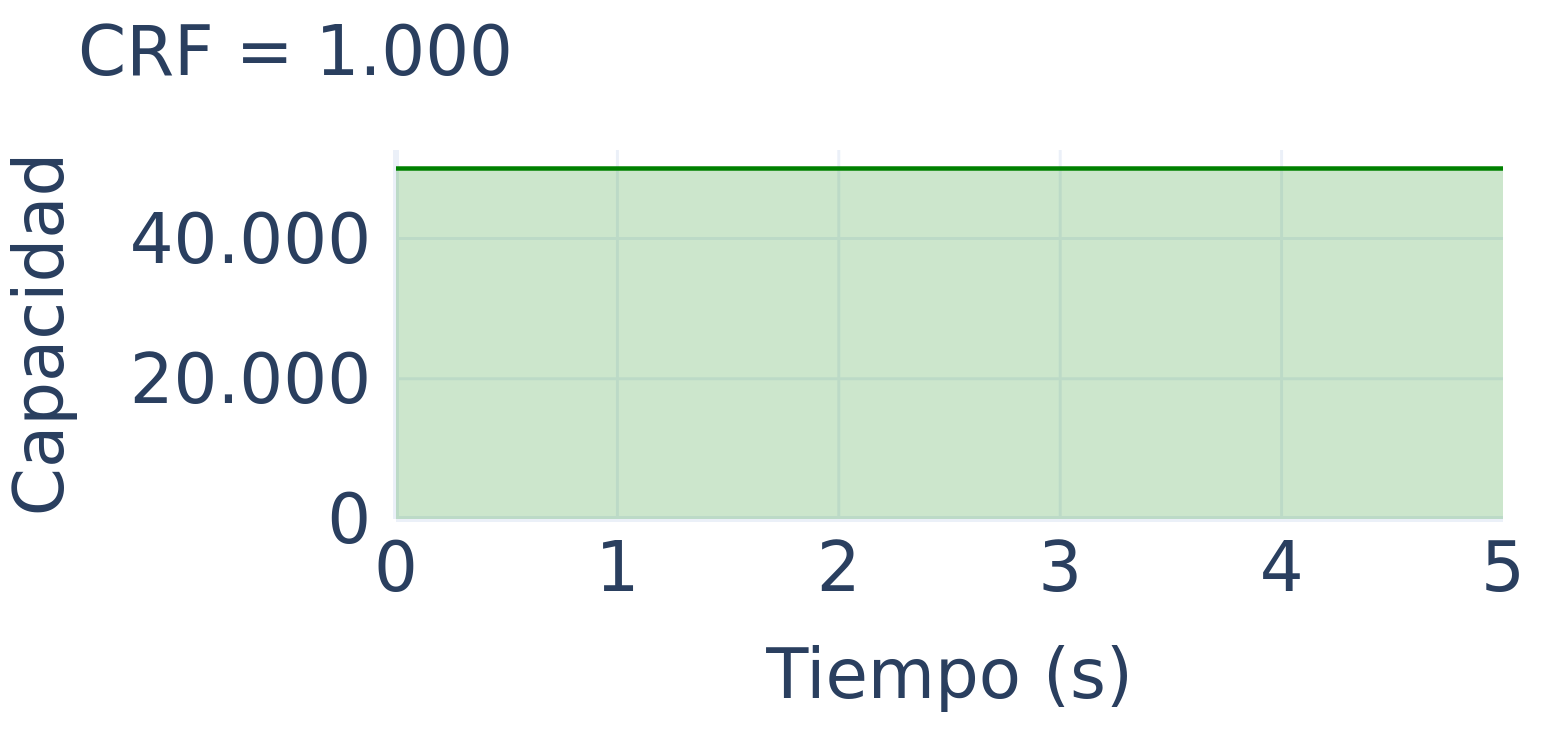
\includegraphics[width=0.42\textwidth]{fig/capacidad_sendgrid_essentials_k1000_2026-10-25.png}}
\subfigure[MailerSend Hobby, $k = 1$ (1 hora)]{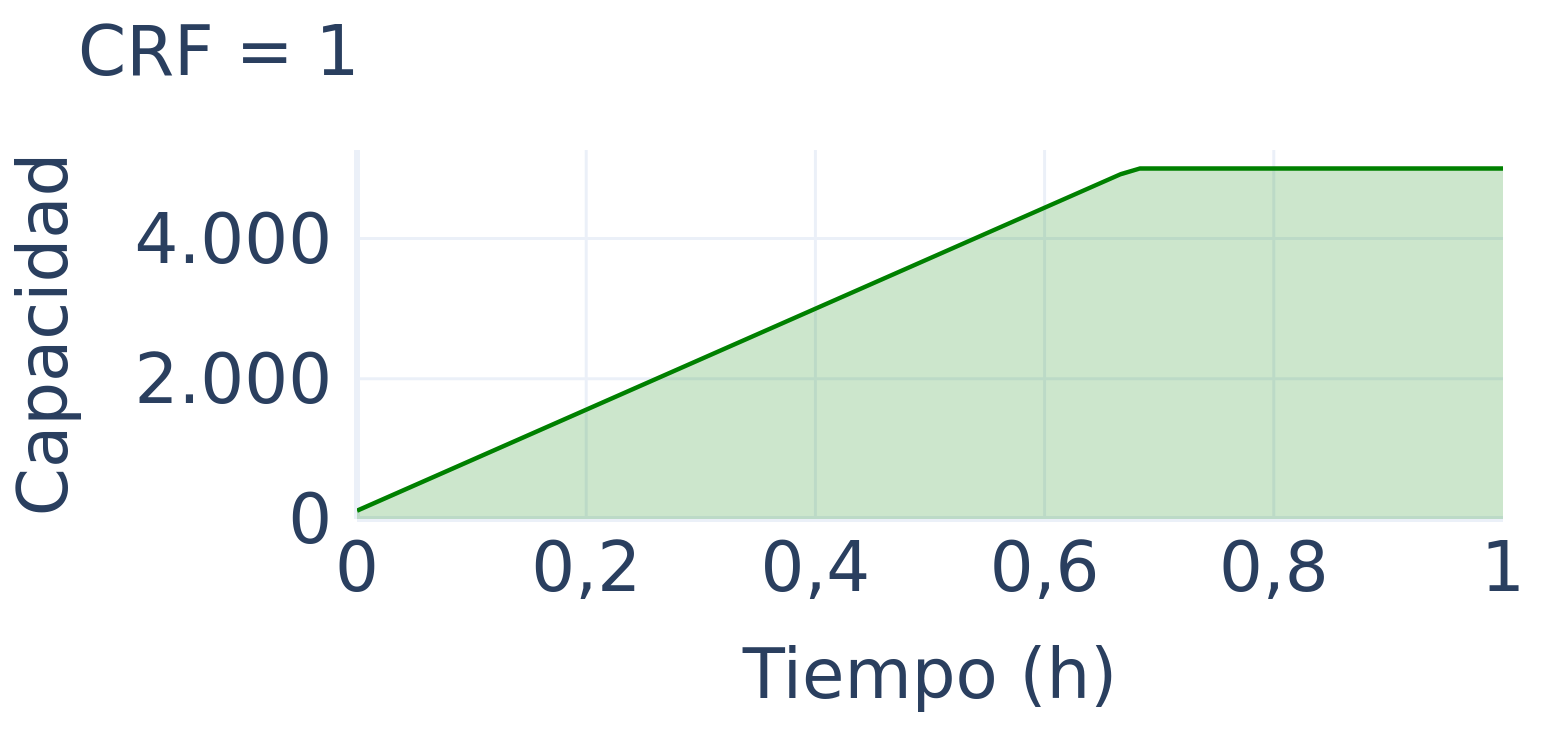
\includegraphics[width=0.42\textwidth]{fig/capacidad_mailersend_hobby_k1_2026-10-25.png}}
\subfigure[Amazon SES, los cuatro planes, $k = 1$ (10 minutos)]{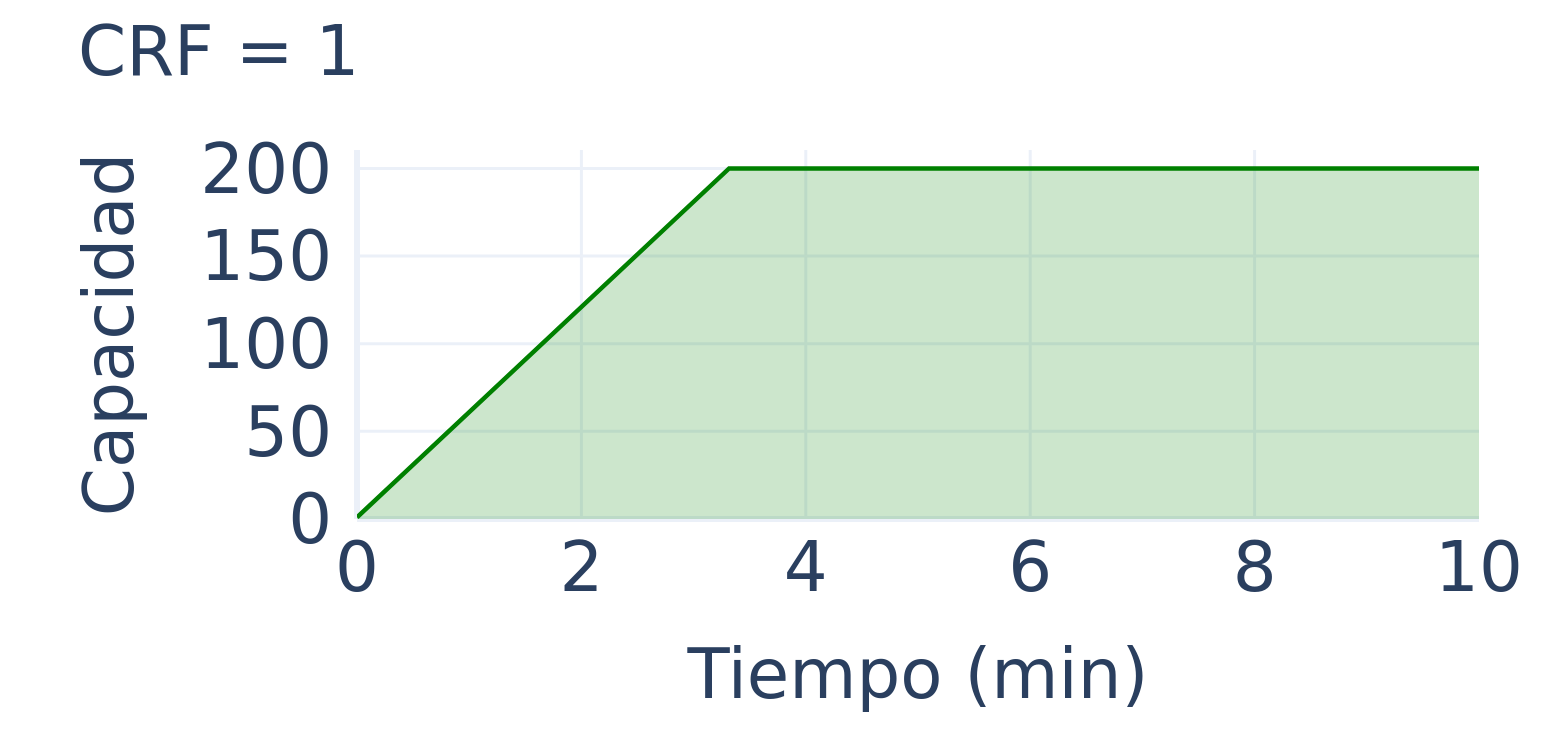
\includegraphics[width=0.42\textwidth]{fig/capacidad_ses_pro_k1_2026-10-25.png}}
\caption[Curva de capacidad $C(t)$ de Resend Pro, SendGrid Essentials 50K, MailerSend Hobby y Amazon SES]{Curva de capacidad $C(t)$ de cuatro planes, dibujada por PRIME4API \citep{prime4apirepo} en local. Entre paréntesis, el intervalo que muestra cada gráfica. Tras el codo, la curva sigue horizontal hasta que la cuota se repone: a los 30 días en Resend, SendGrid y MailerSend, y a las 24 horas en Amazon SES. El área sombreada es la capacidad acumulable.}
\label{fig:capacidad}
\end{figure}

La Figura~\ref{fig:capacidad} muestra la curva de cuatro planes.
La dibuja el propio PRIME4API \citep{prime4apirepo}, ejecutado en local con la misma imagen de contenedor que despliega SPHERE.
El motor lee las Datasheets y su renderizador traza la curva.
Cada gráfica muestra el intervalo que hace visible el codo, porque en una ventana de 30 días el tramo inclinado no se distinguiría de una vertical.
El motor da por enviadas en el instante $t = 0$ las peticiones que el \textit{rate} admite en su primer periodo, un segundo en Resend Pro y un minuto en MailerSend Hobby.
Esa es la primera ráfaga, y por eso el motor da 4.999 segundos en Resend Pro donde el cálculo a mano da 5.000.

En SendGrid Essentials 50K se toma $k = 1.000$, el máximo de destinatarios que el proveedor admite por petición.
Con él la cuota cabe en 50 peticiones, el tramo inclinado dura cinco milésimas de segundo y la curva alcanza la cuota casi desde el origen.
En MailerSend Hobby con $k = 1$ el tramo inclinado sube 120 correos por minuto y el codo llega a los 41 minutos, con una cuota de 5.000 correos al mes.
La gráfica de MailerSend Hobby se pide en correos, la unidad que fija el parámetro \texttt{capacity\_unit} del motor, y por eso no muestra la cuota diaria de peticiones del plan (Apartado~\ref{subsec:evolucion:h1}).
Con esa cuota diaria de 1.000 peticiones, los 5.000 correos con $k = 1$ tardan 4 días y 8 minutos, y no 41 minutos.

En Amazon SES el precio del plan no cambia la curva.
Sus cuatro planes, los tres de la página de precios y la tarifa por uso sin plan, de 0 a 500 USD al mes, devuelven la misma curva, porque la Datasheet les asigna la misma cuota y el mismo caudal.
Son los del entorno de pruebas (\textit{sandbox}), el único para el que Amazon publica cifras.
Toda cuenta nueva de SES empieza en ese entorno, solo puede enviar a direcciones y dominios verificados, y pasa a producción cuando el titular lo pide y Amazon lo aprueba.
En ese entorno el \textit{rate} es de una petición por segundo.
Con un destinatario por petición, la cuota de 200 correos al día se agota en 200 segundos (199 en el motor), y la cuenta no envía nada más hasta que la cuota se repone, a las 24 horas.

El entorno de pruebas es un estado de la cuenta: la condición en que el proveedor tiene la cuenta o su suscripción, con independencia del plan contratado.
El estado de la cuenta reúne el estado de la suscripción, como la cuenta en pruebas o pendiente de aprobación, y la reputación, que separa la cuenta sana de la cuenta en revisión.
En el catálogo, MailerSend baja el \textit{rate} con la cuenta en revisión, y la cuenta de prueba de Mailchimp Transactional tiene su propio caudal de 25 correos por hora.
Una cuenta en estado sano es la que está aprobada y sin restricción por reputación.
El Apartado~\ref{subsec:evolucion:p06} separa el estado de la suscripción de la reputación con el caso de MailerSend.

\section{Lo que publica cada proveedor}\label{sec:limites:publicado}

Las Tablas~\ref{tab:limites-rates} y~\ref{tab:limites-rates-b} dan, plan a plan, la cuota $Q$ y el \textit{rate} $R$ que declara cada Datasheet, con el semáforo de confianza del Apartado~\ref{sec:propuesta:semaforo}.
Un dato va en verde si es literal del proveedor o lo fijó un panel con cuenta propia o un sondeo, en ámbar si exige una lectura que la fuente no hace literal o si dos fuentes oficiales chocan, y en rojo si el proveedor no lo publica.
Con esos pares las tablas calculan el cociente $R \cdot W / Q$ y el tiempo $t_{\min}$ que tarda el \textit{rate} en agotar la cuota, definidos en la Sección~\ref{sec:limites:geometrica}.
Cada cifra tiene su respaldo en el registro de procedencia de su Datasheet, que guarda para cada valor la URL, la fecha de acceso y la cita literal de la fuente.

Cada proveedor reparte sus términos de consumo, el precio y la información de cómo, cuándo, cuánto y dónde se consume, entre varias páginas: la de precios, la de límites de la API, la guía del relé SMTP o unas preguntas frecuentes.
Los párrafos siguientes recogen los casos en que la fuente de la cifra cambia el cálculo, como el \textit{rate} de Postmark, que solo da la cabecera de la respuesta, o el de MailerSend, que baja con la cuenta en revisión.

\textbf{Una cifra que solo se lee en una cabecera y otra que no se puede observar.}
En Postmark el \textit{rate} de la API REST no está publicado, y la documentación describe el error 429 «Rate Limit Exceeded» sin dar el umbral \citep{postmarkapi}.
La cifra sale de la propia API: los cuatro \textit{endpoints} de envío probados devuelven \texttt{ratelimit-\allowbreak limit:~5000} y \texttt{x-ratelimit-\allowbreak limit-second:~5000}, tanto en la respuesta aceptada (200) como en la rechazada por datos no válidos (422).
Que el límite sea por segundo es una lectura del nombre de la cabecera, no un literal del proveedor.
Un sondeo de 200 peticiones no llegó al 429, y la Datasheet adopta 5.000 peticiones por segundo en ámbar para los cuatro planes, aunque solo se observó en la cuenta gratuita.

SendGrid está en el caso opuesto, con una cifra publicada que no se puede observar.
Da 10.000 peticiones por segundo para \texttt{/v3/mail/send} una sola vez, en las preguntas frecuentes del \textit{endpoint} y sin plan ni ámbito\footnote{\url{https://www.twilio.com/docs/sendgrid/for-developers/sending-email/v3-mail-send-faq}. La cita literal está en el \textit{provenance} de \texttt{03\_datos/apis/sendgrid/datasheet.yaml}.}.
La Datasheet la pone en verde porque es un literal del proveedor.
No hay con qué contrastarla: el envío en modo \textit{sandbox} no devuelve cabeceras \texttt{x-ratelimit-*}.
Ese modo es una opción de la petición que la valida sin entregar el correo, y no tiene que ver con el entorno de pruebas de Amazon SES.

\textbf{Un \textit{rate} que cambia con el estado de la cuenta.}
MailerSend ata su \textit{rate} por minuto a la categoría del \textit{endpoint} y al estado de la cuenta \citep{mailersenddocs}.
Con la reputación sana, \texttt{/v1/email} admite 120 peticiones por minuto en los cuatro planes, es decir, $R = 2$, y \texttt{/v1/bulk-email} entre 10 y 30 según el plan.
Con la cuenta bajo revisión, \texttt{/v1/email} baja a 10 peticiones por minuto y \texttt{/v1/bulk-email} a 1.
El sondeo del Apartado~\ref{subsec:evolucion:p06} midió esos 10 en una cuenta sin aprobar, que es un estado de la suscripción distinto de la revisión por reputación para la que el proveedor publica la cifra.
Las 120 peticiones por minuto están publicadas, pero no observadas.

Cada plan de MailerSend tiene además una cuota diaria de peticiones, común a las dos interfaces de envío, la API REST y el relé SMTP.
Va de 100 peticiones en Free a 500.000 en Professional.
Esa cuota no entra en la Ecuación~\eqref{eq:limites-rates} porque cuenta peticiones y no correos, y la Tabla~\ref{tab:limites-rates} la anota aparte.

\begin{table}[H]
\centering
\scriptsize
\setlength{\tabcolsep}{2.5pt}
\begin{tabular}{|l|r|r|r|c|p{3.2cm}|}
\hline
\textbf{API · plan} & \textbf{$R \cdot W$} & \textbf{$Q$} & \textbf{$R \cdot W / Q$} & \textbf{$t_{\min}$ ($k{=}1$ / $k$ máx)} & \textbf{Datos en ámbar o rojo} \\
\hline
Postmark · Free & $1{,}296 \cdot 10^{10}$ & 100 & 129.600.000 & 0,02 s / 0,0004 s & \textit{rate} medido, no publicado \semambar{} \\
\hline
Postmark · Basic & $1{,}296 \cdot 10^{10}$ & 10.000 & 1.296.000 & 2 s / 0,04 s & \textit{rate} \semambar{}, cuota y ventana \semambar{} \\
\hline
Resend · Free (día) & 864.000 & 100 & 8.640 & 10 s / 0,2 s & ventana diaria \semambar{} \\
\hline
Resend · Free (mes) & 25.920.000 & 3.000 & 8.640 & 300 s / 6 s & ventana mensual \semambar{} \\
\hline
Resend · Pro & 25.920.000 & 50.000 & 518,4 & 83,3 min / 100 s & \textit{rate} por defecto \\
\hline
Resend · Scale & 25.920.000 & 100.000 & 259,2 & 2,78 h / 200 s & \textit{rate} por defecto \\
\hline
Resend · Scale 2,5M & 25.920.000 & 2.500.000 & 10,37 & 69,4 h / 83,3 min & volumen contratado no recogido \\
\hline
Resend · Enterprise & n.c. & Custom & n.c. & n.c. & \textit{rate} \semrojo{} \\
\hline
SendGrid · Trial (día) & 864.000.000 & 100 & 8.640.000 & 0,01 s / 1 petición & \textit{rate} no observable \\
\hline
SendGrid · Essentials 50K & $2{,}592 \cdot 10^{10}$ & 50.000 & 518.400 & 5 s / 0,005 s & \textit{rate} no observable \\
\hline
SendGrid · Pro 100K & $2{,}592 \cdot 10^{10}$ & 100.000 & 259.200 & 10 s / 0,01 s & \textit{rate} no observable \\
\hline
SendGrid · Pro 2,5M & $2{,}592 \cdot 10^{10}$ & 2.500.000 & 10.368 & 250 s / 0,25 s & volumen contratado no recogido \\
\hline
SendGrid · Premier & $2{,}592 \cdot 10^{10}$ & Custom & n.c. & n.c. & cuota \textit{custom}, ventana \semambar{} \\
\hline
MailerSend · Free & 5.184.000 & 500 & 10.368 & 250 s / 4 s & ventana \semambar{}, $k$ \semambar{}, \textit{rate} sin observar. Diaria de 100 pet.: 4 d 50 s ($k{=}1$) \\
\hline
MailerSend · Hobby & 5.184.000 & 5.000 & 1.036,8 & 41,7 min / 36 s & $k$ \semambar{}. Diaria de 1.000 pet.: 4 d 8 min ($k{=}1$) \\
\hline
MailerSend · Starter & 5.184.000 & 50.000 & 103,7 & 6,94 h / 6 min & $k$ \semambar{}, lote de 15/min \semverde{} \\
\hline
MailerSend · Starter 1M & 5.184.000 & 1.000.000 & 5,18 & 5,8 d / 2 h & volumen contratado no recogido. Diaria de 100.000 pet.: 10 d ($k{=}1$) \\
\hline
MailerSend · Professional 2M & 5.184.000 & 2.000.000 & 2,59 & 11,6 d / 4 h & volumen contratado no recogido \\
\hline
MailerSend · Starter 1M, rev. & 432.000 & 1.000.000 & 0,43 & $>$ 30 d / 24 h & \textit{rate} de 10/min medido en la cuenta sin aprobar, volumen contratado no recogido \\
\hline
\end{tabular}
\caption[Relación entre \textit{rate} y cuota en Postmark, Resend, SendGrid y MailerSend]{Relación entre \textit{rate} y cuota en Postmark, Resend, SendGrid y MailerSend. $R \cdot W$ va en peticiones por ventana y $Q$ en correos, con un mes de 30 días. $t_{\min}$ se da con $k = 1$ y con el $k$ máximo de cada API: 50 en Postmark y Resend, 1.000 en SendGrid y 70 en MailerSend, este en ámbar. Cuando la cuota se agota en unas pocas peticiones con el $k$ máximo, $t_{\min}$ se da en número de peticiones en lugar de en segundos. La fila «rev.» usa el \textit{rate} de una cuenta de MailerSend bajo revisión. Un volumen contratado «no recogido» lo publica el proveedor y la Datasheet no lo recoge (Apartado~\ref{subsec:evolucion:p01}). Postmark Pro y Platform tienen la misma cuota y el mismo \textit{rate} que Basic, y se omiten. n.c.: no calculable.}
\label{tab:limites-rates}
\end{table}

\textbf{Categorías de \textit{rate} sin plan asignado.}
Brevo da tres cifras para el mismo \texttt{POST /v3/smtp/email}, un \textit{endpoint} de la API REST pese a su nombre: 1.000 peticiones por segundo en la categoría General, 2.000 en Advanced y 6.000 en Extended \citep{brevodocs}.
La página no cierra qué plan cae en cada una, porque una viñeta reserva Advanced a Professional y Enterprise, y el distintivo «Available in» que encabeza la tabla de Advanced enumera los cinco planes, Free incluido.
Los tres valores van en ámbar, y la Tabla~\ref{tab:limites-rates-b} calcula Professional con la cota inferior, la de General, y Enterprise con la superior, la de Extended.

La guía de envío por lotes da otra cifra para el mismo \textit{endpoint}, «Execute the \textit{endpoint} up to 6000 times per hour», 600 veces menos que los 3.600.000 por hora de la categoría General.
La contradicción sigue abierta, y la tabla calcula con la página de categorías.

\textbf{Cifras que solo valen para el entorno de pruebas.}
En Amazon SES las cifras publicadas son las del entorno de pruebas, que es un estado de la cuenta y no un plan: un correo por segundo, 200 correos cada 24 horas y 50 destinatarios por mensaje \citep{sesdocs}.
Para la cuenta de producción, la página de límites escribe que «this number varies based on your specific use case», y la referencia de la API reserva en \texttt{Max24HourSend} el valor $-1$ para una cuota ilimitada, sin decir qué cuenta lo recibe.
Por eso los cuatro planes que la Datasheet toma de la página de precios \citep{sespricing} reciben la cuota y el \textit{rate} del entorno de pruebas.

Hay dos límites de SES que la Datasheet no pudo modelar con ACM2YAML v0.3.
El primero es el tiempo que SES pide esperar tras un rechazo por limitación, que no tiene campo en el esquema.
La página de errores de la cuota de envío da «up to 10 minutes», y la de problemas del relé SMTP, para las peticiones SMTP rechazadas, una serie de esperas de 5, 10 y 30 segundos seguida de 20 minutos.
La primera página cubre también los rechazos SMTP, así que las dos indicaciones chocan.

El segundo es la petición por segundo que la página de límites aplicaba, cuando se consultó, a todas las operaciones salvo SendEmail, SendRawEmail y SendTemplatedEmail, tres nombres de la versión 1 de la API.
La Datasheet modela la versión 2, y el esquema no podía acotar esa cifra a sus operaciones porque la página no decía cuáles cubría: el envío por lotes no estaba ni entre las exentas ni entre las limitadas.
Un sondeo contra \texttt{GET /v2/email/account} aceptó más de cinco veces ese valor sin fijar el umbral (Apartado~\ref{sec:propuesta:casos}).
Desde finales de octubre de 2026 la página exime SendEmail y SendBulkEmail, y con ese texto la cifra ya se puede acotar.

\textbf{Una cifra publicada y otra medida, con ámbitos distintos.}
Mailgun publica una sola cifra de \textit{rate} para su API REST, «1,500 API requests per second per client IP», en las preguntas frecuentes de su sitio comercial y no en la documentación de desarrollador\footnote{\url{https://www.mailgun.com/ai-info/}. La cita literal está en el \textit{provenance} de \texttt{03\_datos/apis/mailgun/datasheet.yaml}.}.
Leída al pie de la letra es un tope por IP de cliente, un ámbito que el esquema no sabe declarar, y la Datasheet la pone en ámbar como caudal del plan.

Lo medido es otro contador, el de la cabecera del envío aceptado: \texttt{x-ratelimit-limit: 80000}, 80.000 peticiones por ventana.
La ventana la abre la primera petición, y dos mediciones de su duración dieron 9,85 y 9,87 segundos.
La misma respuesta trae \texttt{x-recipient-limit: 2000000}, un contador que limita los destinatarios y no las peticiones.
Es el segundo \textit{rate}, $R_d$, que la Sección~\ref{sec:limites:geometrica} admite junto al de peticiones, y no está en la Datasheet porque el esquema admite un solo \textit{rate} por nodo, sea un plan o un \textit{endpoint}.

La Tabla~\ref{tab:limites-rates-b} calcula con $R = 8.000$ peticiones por segundo, una cifra que no publica Mailgun ni trae la cabecera: es el cociente de esas 80.000 peticiones entre los diez segundos a los que la Datasheet redondea la ventana.
La Datasheet declara las 1.500 peticiones por segundo en el plan y el contador de 80.000 en el \textit{endpoint} de envío.
PRIME4API, que suma los límites del plan a los del \textit{endpoint}, aplica las dos cifras a la vez y calcula con la más baja, las 1.500.

La cuota del plan Free de Mailgun tiene dos cifras: la página de precios da 100 correos al día \citep{mailgunpricing} y el panel de la cuenta muestra 3.000 al mes.
Ninguna de las dos fuentes dice si son dos topes simultáneos, y la tabla calcula con ambos.

\textbf{Un caudal en correos por hora.}
Mailchimp Transactional no publica \textit{rate} en peticiones para el envío, y ni sus páginas ni el sondeo dan cabeceras de \textit{rate} \citep{mailchimpdocs}.
El envío de la cuenta de prueba lo gobierna «a fixed hourly quota of 25 emails», y los correos que pasan de ese tope no se rechazan: entran en una cola que se procesa en la hora siguiente.
La Datasheet interpreta ese tope como un \textit{rate} de 25 correos por hora.
La franquicia de 500 correos de esa cuenta no tiene ventana, y en la cuenta de pago la cuota es un bloque de 25.000 correos \citep{mailchimppricing}, con un \textit{rate} que depende de la reputación y no tiene cifra publicada.

\begin{table}[H]
\centering
\scriptsize
\setlength{\tabcolsep}{2.3pt}
\begin{tabular}{|l|r|r|r|c|p{2.7cm}|}
\hline
\textbf{API · plan} & \textbf{$R \cdot W$} & \textbf{$Q$} & \textbf{$R \cdot W / Q$} & \textbf{$t_{\min}$ ($k{=}1$ / $k$ máx)} & \textbf{Datos en ámbar o rojo} \\
\hline
Brevo · Free (día) & 86.400.000 & 300 & 288.000 & 0,3 s / $<$ 1 pet. & \textit{rate} \semambar{}, hora del reinicio diario \semrojo{} \\
\hline
Brevo · Starter & $2{,}592 \cdot 10^{9}$ & 5.000 & 518.400 & 5 s / 3 pet. & \textit{rate} \semambar{}, $k$ \semambar{}, 99 destinatarios con adjunto \\
\hline
Brevo · Standard & $2{,}592 \cdot 10^{9}$ & 5.000 & 518.400 & 5 s / 3 pet. & ídem Starter, misma cuota y distinto precio \\
\hline
Brevo · Professional & $2{,}592 \cdot 10^{9}$ & 150.000 & 17.280 & 150 s / 75 pet. & categoría Advanced sin atribuir \semambar{} \\
\hline
Brevo · Professional 10M & $2{,}592 \cdot 10^{9}$ & 10.000.000 & 259,2 & 2 h 47 min / 5.000 pet. & volumen contratado no recogido \\
\hline
Brevo · Enterprise & $1{,}5552 \cdot 10^{10}$ & Custom & n.c. & n.c. & categoría Extended \semambar{} \\
\hline
SES · pruebas & 86.400 & 200 & 432 & 200 s / 4 s & ventana de la cuota \semrojo{}, no es cuota de plan \\
\hline
SES · producción & n.c. & no publicada & n.c. & n.c. & cuota \semrojo{} y \textit{rate} \semrojo{} \\
\hline
Mailgun · Free (día) & 691.200.000 & 100 & 6.912.000 & 0,0125 s / $<$ 1 pet. & una o dos cuotas, sin decidir \semambar{}, hora de reposición \semrojo{} \\
\hline
Mailgun · Free (mes) & $2{,}0736 \cdot 10^{10}$ & 3.000 & 6.912.000 & 0,375 s / $<$ 1 pet. & ídem, la diaria por 30 da la mensual \\
\hline
Mailgun · Basic & $2{,}0736 \cdot 10^{10}$ & 10.000 & 2.073.600 & 1,25 s / 0,05 s & ventana del \textit{rate} fuera del esquema \semambar{} \\
\hline
Mailgun · Foundation & $2{,}0736 \cdot 10^{10}$ & 50.000 & 414.720 & 6,25 s / 0,25 s & ídem, \textit{rate} no atribuido por plan \semambar{} \\
\hline
Mailgun · Scale & $2{,}0736 \cdot 10^{10}$ & 100.000 & 207.360 & 12,5 s / 0,5 s & ídem \\
\hline
Mailgun · Scale 2,5M & $2{,}0736 \cdot 10^{10}$ & 2.500.000 & 8.294,4 & 312,5 s / 12,5 s & volumen contratado no recogido \\
\hline
Mailchimp · prueba & en correos/h & 500 & no formable & 20 h (cualquier $k$) & cuota sin ventana \semrojo{}, $k$ sin tope \semrojo{} \\
\hline
Mailchimp · bloque de pago & sin cifra & 25.000 & no formable & n.c. & \textit{rate} sin publicar, ventana del bloque \semambar{} \\
\hline
\end{tabular}
\caption[Relación entre \textit{rate} y cuota en Brevo, Amazon SES, Mailgun y Mailchimp]{Relación entre \textit{rate} y cuota en Brevo, Amazon SES, Mailgun y Mailchimp, con las convenciones de la Tabla~\ref{tab:limites-rates}. El $k$ máximo vale 2.000 en Brevo (en ámbar), 50 en SES y 1.000 en Mailgun. El \textit{rate} de Mailgun es el de la cabecera del envío, 80.000 peticiones en una ventana medida de unos diez segundos. Su $R = 8.000$ es el cociente de esas 80.000 peticiones entre los diez segundos a los que la Datasheet redondea la ventana, y no una cifra publicada. Su $t_{\min}$ con $k$ máximo lo gobierna el contador de 2.000.000 de destinatarios sobre la misma ventana. Las dos filas de SES son estados de la cuenta y valen para los cuatro planes. Con adjunto, Brevo baja el tope a 99 destinatarios por petición. Mailchimp declara su \textit{rate} en correos por hora, y por eso no tiene $R \cdot W$. n.c.: no calculable.}
\label{tab:limites-rates-b}
\end{table}

\textbf{La especificación formal dice menos que la prosa.}
La especificación formal de una API es su descripción legible por máquina: un fichero OpenAPI o Swagger que enumera cada ruta con sus parámetros y sus respuestas.
La de SendGrid, en el repositorio \texttt{twilio/sendgrid-oai}, no menciona los \textit{rates} ni el tope de \texttt{to}, y el tope de 1.000 destinatarios por petición, que suma \texttt{to}, \texttt{cc} y \texttt{bcc}, solo aparece en la referencia en prosa \citep{sendgriddocs}.
La de MailerSend, publicada en SwaggerHub, tampoco declara el tope de \texttt{to} ni la respuesta 429 \citep{mailersenddocs}.
La de Brevo, una definición Swagger de 207 rutas, no menciona el \textit{rate} ni una vez \citep{brevodocs}.

Amazon SES publica sus límites en cuatro documentos: la página de límites, la referencia de la operación de envío, la especificación formal de la versión 2 y la guía del relé SMTP \citep{sesdocs}.
En una tabla de doce límites por esos cuatro documentos, de la cuota diaria a la espera tras el rechazo, quedan vacías 32 de las 48 celdas, y la columna de la especificación formal lo está entera.
Una Datasheet construida solo desde la especificación formal recogería menos límites que la construida desde la prosa en esas cuatro APIs, y la comparación no se hizo en las otras cuatro.

\section{Lo que enseña el catálogo}
\label{sec:limites:catalogo}

Las Tablas~\ref{tab:limites-rates} y~\ref{tab:limites-rates-b} recogen el caudal, la cuota y la ventana de cada API, y de ellas salen seis afirmaciones sobre la relación entre límites de uso y \textit{rates}.
Cada afirmación se cuenta sobre las ocho APIs y no sobre sus planes, para que una API con cinco planes no pese cinco veces.
El recuento reparte las ocho en cuatro grupos, que se escriben siempre en este orden: a favor, en contra, no comprobable y no aplica.
Una API cuenta a favor cuando su Datasheet tiene el dato que la afirmación necesita y ese dato va en la dirección enunciada.
Cuenta en contra cuando tiene el dato y apunta al lado opuesto, y entonces es un contraejemplo y se nombra.

Los otros dos grupos separan el dato que falta de la afirmación que no se puede plantear.
Una API es no comprobable cuando la afirmación tiene sentido en ella pero ningún hecho recogido aporta el dato, y en ese caso nunca suma a favor.
No aplica cuando la afirmación presupone una estructura que la API no tiene, como los planes en Mailchimp Transactional o la cuota incluida en Amazon SES.

El cociente $R \cdot W / Q$ es el de la Sección~\ref{sec:limites:geometrica}: cuántas veces cabe la cuota en lo que el \textit{rate} admite durante su ventana.
Como se calcula con un destinatario por petición ($k = 1$), es una cota inferior, porque enviar a varios destinatarios en cada petición solo puede agrandarlo.

La primera afirmación es que, con la cuenta en estado sano, la cuota es la restricción activa en toda API cuya Datasheet lleva \textit{rate} y cuota con valor.
El recuento es de seis a favor, ninguna en contra, una no comprobable y una que no aplica.
El cociente $R \cdot W / Q$ va de 103,7 en MailerSend Starter a 129.600.000 en el plan Free de Postmark, es decir, de dos a ocho órdenes de magnitud.
Con los volúmenes contratados que el proveedor publica y la Datasheet no recoge, el mínimo baja a 2,59 en MailerSend Professional 2M, algo más del doble.

La no comprobable es Amazon SES, porque fuera del entorno de pruebas el proveedor no publica ni el \textit{rate} ni la cuota, que cada cuenta recibe al obtener el acceso de producción.
La que no aplica es Mailchimp Transactional, que no tiene planes y cuya franquicia de prueba de 500 correos no caduca ni se renueva.
Sin ventana en la cuota, el cociente no está definido.
Con 25 correos por hora, agotar esa franquicia lleva veinte horas, así que en esta API el tiempo lo pone el caudal.

En esas seis APIs el \textit{rate} del cociente sale de fuentes distintas, recogidas en la Sección~\ref{sec:limites:publicado}.
Solo MailerSend lo publica para todos sus planes, con 120 peticiones por minuto, y Resend publica un valor por defecto por equipo.
Postmark lo devuelve en la cabecera de respuesta, y la de Mailgun da 80.000 peticiones por una ventana medida de unos diez segundos, que la Tabla~\ref{tab:limites-rates-b} divide para obtener 8.000 por segundo.
SendGrid lo da en unas preguntas frecuentes sin plan, y Brevo no dice qué plan cae en cada categoría.
Para dimensionar un volumen de envío, el \textit{rate} puede ignorarse en seis de las ocho APIs mientras la cuenta esté sana, y en Amazon SES la pregunta no tiene respuesta antes de abrir la cuenta.

La segunda afirmación tiene dos mitades que se cuentan aparte: el \textit{rate} del envío individual no varía con el plan, y lo que el plan compra es cuota.
La primera mitad se limita al envío individual porque MailerSend publica para el envío por lotes, \texttt{/v1/bulk-email}, un caudal que sube con el plan: 10 peticiones por minuto en Hobby, 15 en Starter y 30 en Professional.
Esa mitad queda en tres a favor, una en contra, dos no comprobables y dos que no aplican.
Las tres a favor son Resend, SendGrid y MailerSend.
Resend publica un valor por defecto por equipo, SendGrid publica 10.000 peticiones por segundo sin condición de plan y MailerSend publica 120 peticiones por minuto en \texttt{/v1/email} para sus cuatro planes.

El contraejemplo es Brevo, con las tres categorías de caudal para el mismo \textit{endpoint} de envío que recoge la Sección~\ref{sec:limites:publicado}.
Pasar de la categoría General a la Extended multiplica por seis el caudal del envío individual, que así puede crecer al subir de plan.
El dato va en ámbar (\semambar{}) porque la página no dice qué plan cae en cada categoría.
Postmark y Mailgun son no comprobables, porque su caudal de envío se observó en la cabecera de una sola cuenta gratuita y la Datasheet lo extiende a todos los planes por falta de dato.
La mitad no aplica a Amazon SES, cuyo único caudal publicado es el del entorno de pruebas, un estado de la cuenta y no un plan.
Tampoco aplica a Mailchimp Transactional, que no tiene planes y fija el caudal según su reputación.

La segunda mitad queda en seis a favor y dos que no aplican.
Las seis a favor son Postmark, Resend, SendGrid, MailerSend, Brevo y Mailgun, cuya cuota crece con el precio del plan, en Brevo de 300 correos al día a diez millones al mes.
En Brevo el plan compra además caudal de envío individual, y en MailerSend, caudal de envío por lotes.
En Amazon SES el plan no compra volumen, porque ningún plan incluye cuota: los 200 correos al día del entorno de pruebas valen igual para los cuatro planes, que compran funciones y tramos de precio unitario \citep{sespricing}.
En Mailchimp Transactional no hay planes, y lo que se compra es la propia unidad de volumen, el bloque de 25.000 correos, a un precio que baja de 20 a 10 USD por bloque \citep{mailchimppricing}.

La tercera afirmación es que el \textit{rate} que publica el proveedor coincide con el que devuelve la API en sus cabeceras o con el que mide un sondeo.
El recuento es de cuatro a favor, ninguna en contra, cuatro no comprobables y ninguna que no aplique.
Las cuatro que coinciden publican el valor con su ámbito escrito: Resend lo da por equipo, MailerSend por estado de la cuenta, Brevo ruta a ruta y Mailchimp Transactional para la cuenta de prueba.
La cabecera del envío de Brevo devolvió las 1.000 peticiones por segundo de su tabla General, y en Mailchimp Transactional la documentación, el panel y la medición coinciden en 25 correos por hora.

En MailerSend la coincidencia es de valor y no de estado.
Las 10 peticiones por minuto que el proveedor publica para la cuenta en revisión son las que el sondeo midió en una cuenta sin aprobar, que es otro estado, y las 120 de la cuenta sana siguen sin observar.

Dos de esas coincidencias tienen una segunda cifra al lado.
En Brevo la coincidencia vale solo para la categoría General, porque su guía de envío por lotes da para el mismo \textit{endpoint} 6.000 peticiones por hora, 600 veces menos.
En Resend, la Datasheet de ejemplo que publica el repositorio de la guía de ACM2YAML, fechada en febrero de 2026, fija 2 peticiones por segundo \citep{apisconsumptionmodel}, y la documentación consultada en agosto de 2026 publica 10 \citep{resenddocs}.
Las capturas de su página de límites en Wayback Machine muestran que cambió la oferta: 2 por segundo hasta marzo de 2026, 5 entre abril y julio, y 10 desde agosto.

Las cuatro no comprobables carecen de una cifra publicada y observada para el mismo \textit{endpoint} y el mismo ámbito.
Postmark no publica \textit{rate} y devuelve 5.000 en la cabecera de cada respuesta.
SendGrid publica 10.000 peticiones por segundo para un \textit{endpoint} de envío que, en modo \textit{sandbox}, no devuelve cabeceras, y en los de lectura devuelve 600 y 6 en \texttt{X-RateLimit-Limit}, valores que ninguna página documenta.
Amazon SES no publica su caudal de producción.

En Mailgun, la cifra publicada y la medida tienen ámbitos distintos.
Sus preguntas frecuentes dan 1.500 peticiones por segundo por IP de cliente para toda la API, y la cabecera del envío cuenta otro contador, 80.000 peticiones por una ventana de unos diez segundos (unas 8.000 por segundo si se dividen).
La medición no dice cuál de los dos rige en el envío, así que no contradice la cifra publicada.

La cabecera de respuesta tampoco es una señal fiable en todo el catálogo.
Amazon SES no emite ninguna cabecera de caudal, y sus nueve respuestas 429 medidas no traen \texttt{Retry-After}, la cabecera que dice cuánto esperar antes de reintentar.
Mailchimp Transactional no emite cabecera de caudal en ninguna respuesta del sondeo ni la menciona en ninguna página oficial.
Mailgun la emite solo en un POST aceptado, así que leer el caudal le cuesta al cliente un envío.

Donde la cabecera llega, la documentación no siempre la describe bien.
Brevo afirma que llega en todas las respuestas, y en la medición llegó en una respuesta de error 400 y no en dos respuestas correctas 200.
En SendGrid, \texttt{X-RateLimit-Reset} trae en tres \textit{endpoints} un valor de una o dos cifras (6, 9 y 58), que se lee como los segundos que faltan, y en otros tres una marca de tiempo Unix.
La documentación solo muestra la segunda forma \citep{sendgridratelimits}.
Una herramienta que lea esa cabecera para calcular cuándo reintentar encuentra el mismo nombre con dos formas de valor y ningún aviso.

La alternativa a la cabecera es un \textit{endpoint} que informa de la capacidad restante de la cuenta sin gastar cuota, y cuatro de las ocho APIs lo tienen, aunque el de Brevo da el saldo y no el límite.
Amazon SES devuelve en un \texttt{GET} la cuota de 24 horas y el caudal máximo de envío de la cuenta, y su documentación lo señala como la vía para conocerlas.
Mailchimp Transactional devuelve la cuota horaria junto a la reputación en \texttt{POST /users/info}, y MailerSend tiene \texttt{GET /v1/api-quota} \citep{mailersenddocs}.
El \texttt{GET /v3/account} de Brevo devuelve el saldo de correos y el periodo exacto del ciclo, pero ninguno de sus campos es de límite.

Postmark, Resend, SendGrid y Mailgun no tienen ninguno, y en ellas el cliente conoce su capacidad restante después de gastarla o no llega a conocerla.
Donde existe, el \textit{endpoint} tampoco garantiza un dato al día.
En MailerSend, once horas y veinticuatro minutos después de la medianoche que repone la cuota diaria, seguía sirviendo el saldo del día anterior.

La cuarta afirmación es que el proveedor publica un tope de destinatarios por petición, el valor máximo del factor $k$ con el que se pasa del \textit{rate}, que cuenta peticiones, a la cuota, que cuenta correos.
El recuento es de siete a favor, una en contra, ninguna no comprobable y ninguna que no aplique, porque siete APIs publican ese tope y una no.
Postmark, Resend y Amazon SES admiten 50 destinatarios por petición, MailerSend 70, SendGrid 1.000, Mailgun 1.000 por lote y Brevo 2.000.
El contraejemplo es Mailchimp Transactional, que escribe que no hay limitación de destinatarios y que el JSON de la llamada debe pesar menos de 10 MB \citep{mailchimpdocs}.
Ahí la cota de una llamada está en megabytes, y no hay $k$ que pase de una unidad a la otra.

Cinco de los siete topes están verificados por sondeo: los de Postmark, Resend, SendGrid y Mailgun, y el de la cuenta sin aprobar de MailerSend.
En Mailgun el destinatario 1.001 devuelve un error 400 que nombra el máximo de 1.000.
En Brevo no hubo sondeo de destinatarios, y el tope de Amazon SES sale de su página de cuotas, que lo define como la suma de \texttt{To}, \texttt{Cc} y \texttt{Bcc} \citep{sesdocs}.
En Amazon SES una petición de 50 destinatarios consume la cuarta parte de la cuota diaria del entorno de pruebas, y en Brevo una de 2.000 equivale a casi siete veces la cuota diaria del plan Free.

El factor $k$ solo conecta las dos magnitudes si cada destinatario descuenta una unidad de cuota.
De las cuatro APIs en las que esa equivalencia está sostenida (Sección~\ref{sec:limites:geometrica}), Resend y SendGrid la publican, y en Brevo y Amazon SES salió de medir.
En Brevo, el saldo de la cuenta bajó de 300 a 298 tras una petición con dos destinatarios.
En Amazon SES, el contador marcó 5 sobre 200 tras cuatro mensajes con cinco destinatarios, porque uno llevaba la misma dirección en \texttt{to} y en \texttt{cc}.
Ese recuento descarta a la vez que la unidad sea el mensaje y que el proveedor deduplique direcciones, porque cualquiera de las dos habría dado cuatro.
En Postmark, MailerSend, Mailgun y Mailchimp Transactional esa equivalencia es una suposición que ningún dato confirma.

La quinta afirmación es que el proveedor no publica un caudal propio de cada plan ni cuándo se repone la cuota.
En la mitad que trata del caudal del envío individual, el recuento es de siete a favor, una en contra, ninguna no comprobable y ninguna que no aplique.
Un caudal común a todos los planes, como las 120 peticiones por minuto de MailerSend, cuenta a favor, porque no es propio de ningún plan.
El contraejemplo es Brevo, la única que pone una cifra de ese caudal junto a una categoría de plan.
Amazon SES cuenta a favor porque no publica el caudal de producción.
El envío por lotes de MailerSend, con 10, 15 y 30 peticiones por minuto según el plan, queda fuera de esta mitad por el mismo motivo que en la segunda afirmación.

Cuatro de las siete Datasheets declaran de formas distintas el caudal que el proveedor no liga a un plan.
La de Amazon SES deja vacío el bloque de caudal, la de Mailgun referencia un único valor desde sus cuatro planes y la de MailerSend toma las 120 peticiones por minuto como valor por defecto.
La de Mailchimp Transactional repite el caudal como estado de la cuenta en sus tres \textit{endpoints} de envío.

La otra mitad de la quinta afirmación, la de la ventana de la cuota, queda en ocho a favor.
Ninguna API tiene esa ventana en verde si cada una se clasifica por el peor semáforo de sus cuotas: cuatro están en rojo (\semrojo{}) y cuatro en ámbar (\semambar{}).
SendGrid es la que más se acerca, porque publica la medianoche UTC y el periodo de facturación, y solo la ventana de su plan Premier queda en ámbar.

Los cuatro rojos responden a tres causas.
Mailgun y Brevo dan valor y periodo para las cuotas de su plan Free, pero ninguna fuente fecha su reposición.
Amazon SES describe su cuota diaria como deslizante en una página, es decir, que en cada envío cuenta lo enviado en las 24 horas anteriores, y como fija en otra, en la que hay que esperar al siguiente periodo de 24 horas.
El campo se deja vacío a propósito.
Mailchimp Transactional escribe que su franquicia no caduca ni se renueva, mientras ACM2YAML v0.3 exige un periodo en toda cuota.
En esas cuatro APIs, quien integra la API no puede calcular cuándo se repone su cuota sin observarlo en su propia cuenta.

La ventana del caudal no la declara ninguna de las ocho, y dos sondeos la acotaron.
En Brevo la ruta \texttt{GET /v3/smtp/emails}, que consulta la actividad de envío, volvió a admitir peticiones antes de cumplirse un segundo desde la primera de la serie, y con una sola muestra no se distingue una ventana fija alineada con el reloj de una reposición gradual.
En Mailgun la ventana dura entre 9,85 y 9,87 segundos, la abre la primera petición y no es deslizante, y ninguno de los tres tipos de ventana que admite ACM2YAML v0.3 (deslizante, fija a la medianoche UTC y fija al ciclo de facturación) la describe.

La sexta afirmación es que el estado de la cuenta condiciona la capacidad, con independencia del plan.
El recuento es de seis a favor, dos en contra, ninguna no comprobable y ninguna que no aplique.
Son las seis APIs en que la capacidad depende del estado de la cuenta y no del plan, recogidas como F-18 en el Apartado~\ref{subsec:evolucion:p06}.
Ese apartado describe el caso de MailerSend y la extensión que se propone para modelar el estado de la suscripción.
Solo MailerSend da una cifra para cada estado: 120 peticiones por minuto en \texttt{/v1/email} con la cuenta sana y 10 con la cuenta en revisión.

Las otras cinco a favor son Amazon SES, Mailchimp Transactional, Postmark, Resend y Mailgun.
Amazon SES publica los topes del entorno de pruebas y no los de producción.
Mailchimp Transactional fija 25 correos por hora en la cuenta de prueba y ata la de pago a su reputación.
Postmark limita la cuenta en modo de prueba a 100 correos y a dominios verificados, y con la cuenta pendiente de aprobación rechazó con el código 412 cada mensaje a otro dominio.
Resend sube su valor por defecto de 10 peticiones por segundo a los remitentes de confianza, sin decir cuánto ni qué umbral los define.
Mailgun eleva el caudal a medida que crece la reputación de envío, sin una sola cifra.
Ninguna de las seis publica el umbral que dispara el cambio de estado.

Las dos en contra son SendGrid y Brevo.
En SendGrid el único estado que cambia la capacidad es el fin de la prueba gratuita, que es la caducidad de un plan y no un estado de la cuenta.
En Brevo lo que cambia el caudal es la categoría del acuerdo comercial y no el estado de la cuenta, y para la cuenta sin aprobar no hay cifra.
ACM2YAML v0.3 ya cubre parte de esos estados con sus alias de estado, nombres bajo un \textit{endpoint} que agrupan los límites de cada estado, como el \texttt{sandbox} de Amazon SES (Apartado~\ref{subsec:evolucion:p06}).

Fuera de las seis afirmaciones, el catálogo muestra qué pasa con el envío que supera la cuota.
Cinco de las ocho APIs cobran un sobrecoste por cada correo que pasa de la cuota del plan, y en las cinco su precio baja con el volumen.
Los tramos de Postmark y Resend ya se recogieron en el Apartado~\ref{subsec:evolucion:p01}, donde un mismo plan cambia de sobrecoste con el volumen contratado.
En las otras tres, MailerSend va de 1,50 a 0,50 USD por cada mil correos y Mailgun de 1,80 a 0,40 USD \citep{mailgunpricing}.
SendGrid fija el sobrecoste por correo, y llevado a mil correos va de 1,30 a 0,50 USD.

Las tres APIs sin sobrecoste ponen algo distinto en su lugar.
Brevo niega que haya cargos adicionales y sube de plan automáticamente cuando crece el número de contactos \citep{brevopricing}.
Amazon SES no tiene cuota incluida que exceder, y sus tramos de precio bajan con el volumen sin corte ni penalización \citep{sespricing}.
Mailchimp Transactional detiene el envío al agotar el bloque, y lo que ocupa el lugar del sobrecoste es comprar otro.

En el borde de la cuota hay tres comportamientos documentados.
Amazon SES rechaza la llamada que pasa de la cuota de 24 horas de la cuenta y descarta el mensaje sin ponerlo en cola ni reintentarlo.
SendGrid en su prueba gratuita, MailerSend en el plan Free y Mailchimp Transactional al agotar los bloques detienen el envío.
Brevo retiene en cola hasta 1.000 correos por encima de la cuota diaria y no entrega los que pasan de esa cifra.
Los Apartados~\ref{subsec:evolucion:p07} y~\ref{subsec:evolucion:p09} recogen las dos propuestas que salen de este borde: el tope de diez veces el volumen del plan que SendGrid impone al sobrecoste y la cola con la que Brevo retiene los correos tras agotar la cuota.

Ninguna de las seis afirmaciones se cumple entera en las ocho APIs, y Mailchimp Transactional y Amazon SES quedan fuera de al menos dos de ellas.

\section{Lo que responde PRIME4API}
\label{sec:limites:prime4api}

Dos de los cálculos de la Sección~\ref{sec:limites:geometrica}, la restricción activa y el tiempo mínimo $t_{\min}$, corresponden a operaciones de PRIME4API, el motor de análisis de la capacidad de Gavira Sánchez \citep{gavira2026tfm}, que las resuelve para cada valor del factor $k$.
Se han ejecutado contra el motor como servicio REST en local, sobre las ocho Datasheets, con la petición y la respuesta de cada pregunta archivadas en el repositorio de datos.
Sus respuestas coinciden con el cálculo a mano salvo por tres convenciones de conteo, por los volúmenes contratados que la Datasheet no declara y por el caudal que toma en Mailgun.
El motor no pasa a correos la cuota diaria en peticiones de MailerSend, y sobre la Datasheet de Mailchimp Transactional no responde a la pregunta del tiempo mínimo.

\subsection{Correspondencia con el cálculo a mano}

La restricción activa a consumo uniforme corresponde a la operación que comprueba si una demanda con \textit{rate} y cuota puede sostenerse durante un período.
El tiempo mínimo $t_{\min}$ de la Ecuación~\eqref{eq:limites-rates} corresponde a la que calcula cuánto tarda en agotarse una cuota, y es lo que Gavira Sánchez llama umbral de agotamiento \citep{gavira2026tfm}.

El factor de equilibrio $k^{*} = Q/(R \cdot W)$ es el número de destinatarios por petición con el que el \textit{rate} y la cuota se agotan a la vez.
Una de las diez preguntas de análisis de Gavira Sánchez pide el CRF con el que dos cuotas de un mismo plan o \textit{pricing} se agotan a la vez \citep{gavira2026tfm}.
Aquí se aplica al par \textit{rate} y cuota, tratando el \textit{rate} como un límite con ventana de un segundo.
El motor no calcula $k^{*}$ con una operación propia: devuelve el tiempo de agotamiento de cada límite para cada $k$, y $k^{*}$ se deriva de esos tiempos.

El factor de equilibrio es el inverso del cociente $R \cdot W / Q$ de las Tablas~\ref{tab:limites-rates} y~\ref{tab:limites-rates-b}, así que se lee en ellas sin otro cálculo.
Vale 0,0019 en Resend Pro, $1{,}9 \cdot 10^{-6}$ en SendGrid Essentials 50K, 0,00096 en MailerSend Hobby y 0,0023 en el entorno de pruebas de Amazon SES.
Como $k$ cuenta destinatarios y no baja de uno, un $k^{*}$ menor que uno significa que la cuota se agota siempre antes que el \textit{rate}.
Las dos tablas tienen una sola fila con cociente menor que uno, MailerSend Starter 1M con la cuenta bajo revisión del proveedor, y su $k^{*}$ es 2,31.
Ningún plan publicado con la cuenta en estado sano tiene un $k \geq 1$ que iguale los dos límites.

Mailgun sí tiene un $k^{*}$ mayor que uno, pero se da entre sus dos contadores de caudal y no entre caudal y cuota.
Con los 2.000.000 de destinatarios y las 80.000 peticiones por ventana que devuelve su cabecera (Sección~\ref{sec:limites:publicado}), el contador de destinatarios corta antes a partir de 25 destinatarios por petición.
En Mailchimp Transactional la operación no se puede plantear, porque el caudal ya está en correos y $k$ no multiplica nada.

El motor reproduce el cálculo a mano en Resend y SendGrid, con tres convenciones propias.
Cuenta la primera ráfaga en $t = 0$, y por eso da 4.999 segundos en Resend Pro donde a mano salen 5.000.
Abre la ventana siguiente en el instante final de un intervalo, y en $t = 30$ días suma ya la primera ráfaga de esa ventana.
Aplica a cada ventana mensual, y no solo a la primera, la cuota ampliada con el sobrecoste que paga el presupuesto.

Aparte de esas convenciones, el motor solo ve el primer volumen contratado de cada plan, porque la Datasheet no declara más.
Con 50 USD al mes, en Resend Pro y SendGrid Essentials el motor parte del volumen de 50.000 correos y da 83.343 y 83.115 correos, cifras correctas para lo que la Datasheet declara.
Los dos proveedores venden un segundo volumen contratado de 100.000 correos por 35 y 34,95 USD, que la Datasheet solo recoge en el registro de procedencia.
Con ese segundo volumen el mismo presupuesto daría 116.000 y 116.722 correos, de modo que el motor se queda entre un 28 y un 29~\% por debajo por un dato que la Datasheet no declara.

En Brevo y Amazon SES las respuestas del motor solo difieren del cálculo a mano por las tres convenciones.
En Mailgun el motor aplica a la vez la cifra por IP que la Datasheet declara en el plan, 1.500 peticiones por segundo, y el contador de la cabecera del envío, 80.000 peticiones por ventana, y calcula con la primera, más baja.
La Tabla~\ref{tab:limites-rates-b} usa solo el contador, dividido entre diez segundos.
En Mailchimp Transactional no responde a la pregunta del tiempo mínimo para enviar 100.000 correos.

El motor aplica una regla de herencia: suma los límites del plan a los del \textit{endpoint}.
Si la cuota y el \textit{rate} de SendGrid Essentials 50K se declaran en el plan y otra vez en el \textit{endpoint}, con $k = 1.000$ el motor da 100.000 correos a 30 días donde el proveedor publica 50.000.
Por eso las Datasheets del catálogo declaran cada límite una sola vez, en el plan si vale para todos los \textit{endpoints} y en el \textit{endpoint} si es propio.
El validador de formato de este trabajo, el que comprueba los tipos y las referencias de cada Datasheet, falla cuando un límite se repite.
La Figura~\ref{fig:capacidad} es la que devuelve el motor sobre las Datasheets con esa regla aplicada.

\subsection{«No publicado» frente a «sin límite» desde el motor}

Antes de adoptar las 5.000 peticiones por segundo de la cabecera, la Datasheet de Postmark tenía vacío el bloque de los \textit{rates}, \texttt{max\_power}, y muestra qué hace el motor en ese caso.
Con el bloque vacío, el motor responde 0 segundos para agotar la cuota de 10.000 correos del plan Basic.
Para 100.000 correos responde 270 días, que son nueve renovaciones de la cuota mensual, como si el \textit{rate} fuese infinito.
Con el caudal de 5.000 peticiones por segundo medido en la cabecera de respuesta, el motor responde 1 segundo para agotar la cuota (2 a mano, por la convención de la primera ráfaga).
Para los 100.000 correos responde 270 días y 1 segundo.

Con un presupuesto de $10^{9}$ USD, la capacidad a un mes pasa de $1{,}1 \cdot 10^{12}$ correos, que solo acota ese presupuesto porque ningún caudal frena el consumo, a 12.960.005.000.
Esa segunda capacidad es $R \cdot W$ más la primera ráfaga de la ventana siguiente.
Ante un pico de 20.000 correos en una hora, el veredicto es negativo en los cuatro planes, tanto con el bloque vacío como con el caudal declarado.
Lo que cambia es la causa que el motor declara: \texttt{rate\_exceeded} con el bloque vacío, aunque lo que se viola es la cuota, y \texttt{quota\_exceeded} con el caudal declarado.

Tratar como infinito el caudal que el esquema deja vacío es la confusión entre «no publicado» y «sin límite» que la propuesta P-04 quiere impedir con una marca explícita de valor no publicado junto al campo (Apartado~\ref{subsec:evolucion:p04}).

En Amazon SES el plan no cambia la respuesta del motor.
Los cuatro planes devuelven 200 correos al día, una petición por segundo, 1.401 correos en siete días y 6.001 al mes, todo tomado del estado \texttt{sandbox}, el entorno de pruebas.
Ante el mismo pico de 20.000 correos en una hora, el motor responde que no en los cuatro planes con la causa \texttt{rate\_exceeded}.
Aquí la causa es correcta, porque una petición por segundo no sostiene los 5,56 correos por segundo que pide la demanda, y la violación se produce desde el instante cero.

\subsection{Los dos regímenes del sobrecoste}

La pregunta del tiempo mínimo para enviar 100.000 correos tiene dos respuestas en el motor, según reciba o no un presupuesto.
Sin el parámetro \texttt{max\_budget}, el motor trata la cuota con sobrecoste como un corte estricto, que no se puede superar pagando: cuenta renovaciones y mide el tiempo en meses.
En MailerSend Hobby, 100.000 correos tardan así 570 días y 41 minutos, que son diecinueve renovaciones de la cuota de 5.000 correos.
Con un presupuesto que no limita, el motor expande la cuota con el sobrecoste que publica el proveedor, y el tiempo lo fija el caudal: 13 horas y 53 minutos.
Esa cifra no aplica la cuota diaria de 1.000 peticiones del plan, que el motor no pasa a correos (Apartado~\ref{subsec:evolucion:h1}): con ella, los 100.000 correos con $k = 1$ tardan 99 días y 8 minutos.

Los dos tiempos salen de datos del proveedor, y ninguno es una hipótesis de este trabajo.
El segundo tampoco exige elegir un presupuesto, porque a partir de lo que cuestan los 100.000 correos la respuesta deja de cambiar.
En Hobby, 100.000 correos cuestan 149,50 USD: con 149,40 USD el motor sigue respondiendo en días, y con 149,50 USD responde 13 horas y 53 minutos, igual que con mil millones.

La Tabla~\ref{tab:a06-presupuesto} pone los dos regímenes al lado en siete APIs.
En Mailgun Basic el presupuesto baja el tiempo de 100.000 correos de 270 días a 1 minuto y 6 segundos.
Ese tiempo sale del caudal de 1.500 peticiones por segundo por IP que declara la Datasheet, y no del contador de 80.000 peticiones por ventana de unos diez segundos.
En Brevo Starter y en Amazon SES la misma llamada no mueve un segundo, porque sus cuotas no declaran sobrecoste.
La distancia entre las dos columnas llega a seis órdenes de magnitud en Postmark Basic con $k = 1$, de 270 días a 19 segundos.

\begin{table}[H]
\centering
\small
\begin{tabular}{|l|c|r|r|}
\hline
\textbf{API y plan} & \textbf{$k$} & \textbf{Corte estricto} & \textbf{Presupuesto que no limita} \\
\hline
Postmark Basic          & 1     & 270 d 1 s            & 19 s \\
                        & 50    & 270 d                & 0 s \\
\hline
Resend Pro              & 1     & 30 d 1 h 23 min 19 s & 2 h 46 min 39 s \\
                        & 50    & 30 d 1 min 39 s      & 3 min 19 s \\
\hline
SendGrid Essentials 50K & 1     & 30 d 4 s             & 9 s \\
                        & 1.000 & 30 d                 & 0 s \\
\hline
MailerSend Hobby        & 1     & 570 d 41 min         & 13 h 53 min \\
                        & 70    & 570 d                & 11 min \\
\hline
Brevo Starter           & 1     & 570 d 4 s            & 570 d 4 s \\
                        & 2.000 & 570 d                & 570 d \\
\hline
SES Pro (\texttt{sandbox}) & 1  & 499 d 3 min 19 s     & 499 d 3 min 19 s \\
                        & 50    & 499 d 3 s            & 499 d 3 s \\
\hline
Mailgun Basic           & 1     & 270 d 6 s            & 1 min 6 s \\
                        & 1.000 & 270 d                & 0 s \\
\hline
\end{tabular}
\caption[Tiempo mínimo para 100.000 correos con corte estricto y con presupuesto que no limita]{Tiempo mínimo para enviar 100.000 correos en un plan de pago de cada API, respondido por PRIME4API \citep{prime4apirepo} en los dos regímenes. Sin \texttt{max\_budget}, la cuota con sobrecoste se trata como corte estricto y el motor cuenta renovaciones. Con un presupuesto que no limita, el motor la expande y manda el caudal. Brevo y SES son los dos casos sin sobrecoste declarado, y por eso las dos columnas coinciden. Las filas de SES son las del estado \texttt{sandbox}, el único que el proveedor cifra. Mailchimp Transactional no aparece porque el motor no responde a esta pregunta sobre su Datasheet. La fila de Mailgun usa el caudal de 1.500 peticiones por segundo por IP. La fila de MailerSend Hobby no aplica la cuota diaria de 1.000 peticiones del plan (Apartado~\ref{subsec:evolucion:h1}).}
\label{tab:a06-presupuesto}
\end{table}

Nada en la Datasheet dice cuál de los dos regímenes describe el plan.
La cuota lleva su sobrecoste, pero no declara si el proveedor lo cobra sin más, si exige aprobarlo o si lo limita un tope.
El tope de sobrecoste de SendGrid, diez veces el volumen del plan (500.000 correos en Essentials 50K), tendría que entrar en la operación que calcula el importe del sobrecoste, pero la Datasheet no tiene dónde declararlo.
La propuesta P-07, que añade a la cuota un campo para ese tope, lo permite (Apartado~\ref{subsec:evolucion:p07}).
El modo del sobrecoste no tiene campo: es la carencia F-13 de la Tabla~\ref{tab:sinforma}, vista ahora desde el motor, y sigue entre las carencias sin forma fijada.

\subsection{La cuota que no cambia de unidad}
\label{subsec:evolucion:h1}

MailerSend declara en su plan Hobby dos cuotas en unidades distintas: 5.000 correos al mes y 1.000 peticiones al día.
Su \textit{endpoint} de envío declara un \texttt{workload} de hasta 70 destinatarios por petición, y ese factor $k$ es el que el motor usa para pasar de una unidad a otra.
Pedida la curva en correos, la respuesta trae el caudal y la cuota mensual, y no la diaria.
Pedida en peticiones, trae los tres límites: el caudal y la cuota diaria tal cual, y la mensual dividida por $k$.
De las tres conversiones que el factor permite, el motor hace dos.
Multiplica por $k$ el caudal de peticiones para darlo en correos, y divide por $k$ la cuota mensual de correos para darla en peticiones.
La cuota diaria en peticiones no la lleva a correos.

Que el motor no pase la cuota diaria a correos cambia la respuesta.
Con $k = 1$, el motor responde que los 5.000 correos de Hobby se agotan en 41 minutos, mientras que con la cuota diaria de 1.000 peticiones tardarían 4 días y 8 minutos.
La capacidad a un mes con presupuesto sin tope sale de 5.184.120 correos, y con la cuota diaria sería de 30.000.
Con 50 USD de presupuesto el motor devuelve 33.786,67 correos, sin redondear, y con la cuota diaria también saldrían 30.000.
Quien pregunta en correos, que es la unidad del dominio, recibe la cifra optimista.
La Figura~\ref{fig:limites:hobby-peticiones} es la misma llamada pedida en peticiones, y en ella la cuota diaria sí aparece: la curva sube 1.000 cada medianoche durante cinco días.

\begin{figure}[H]
\centering
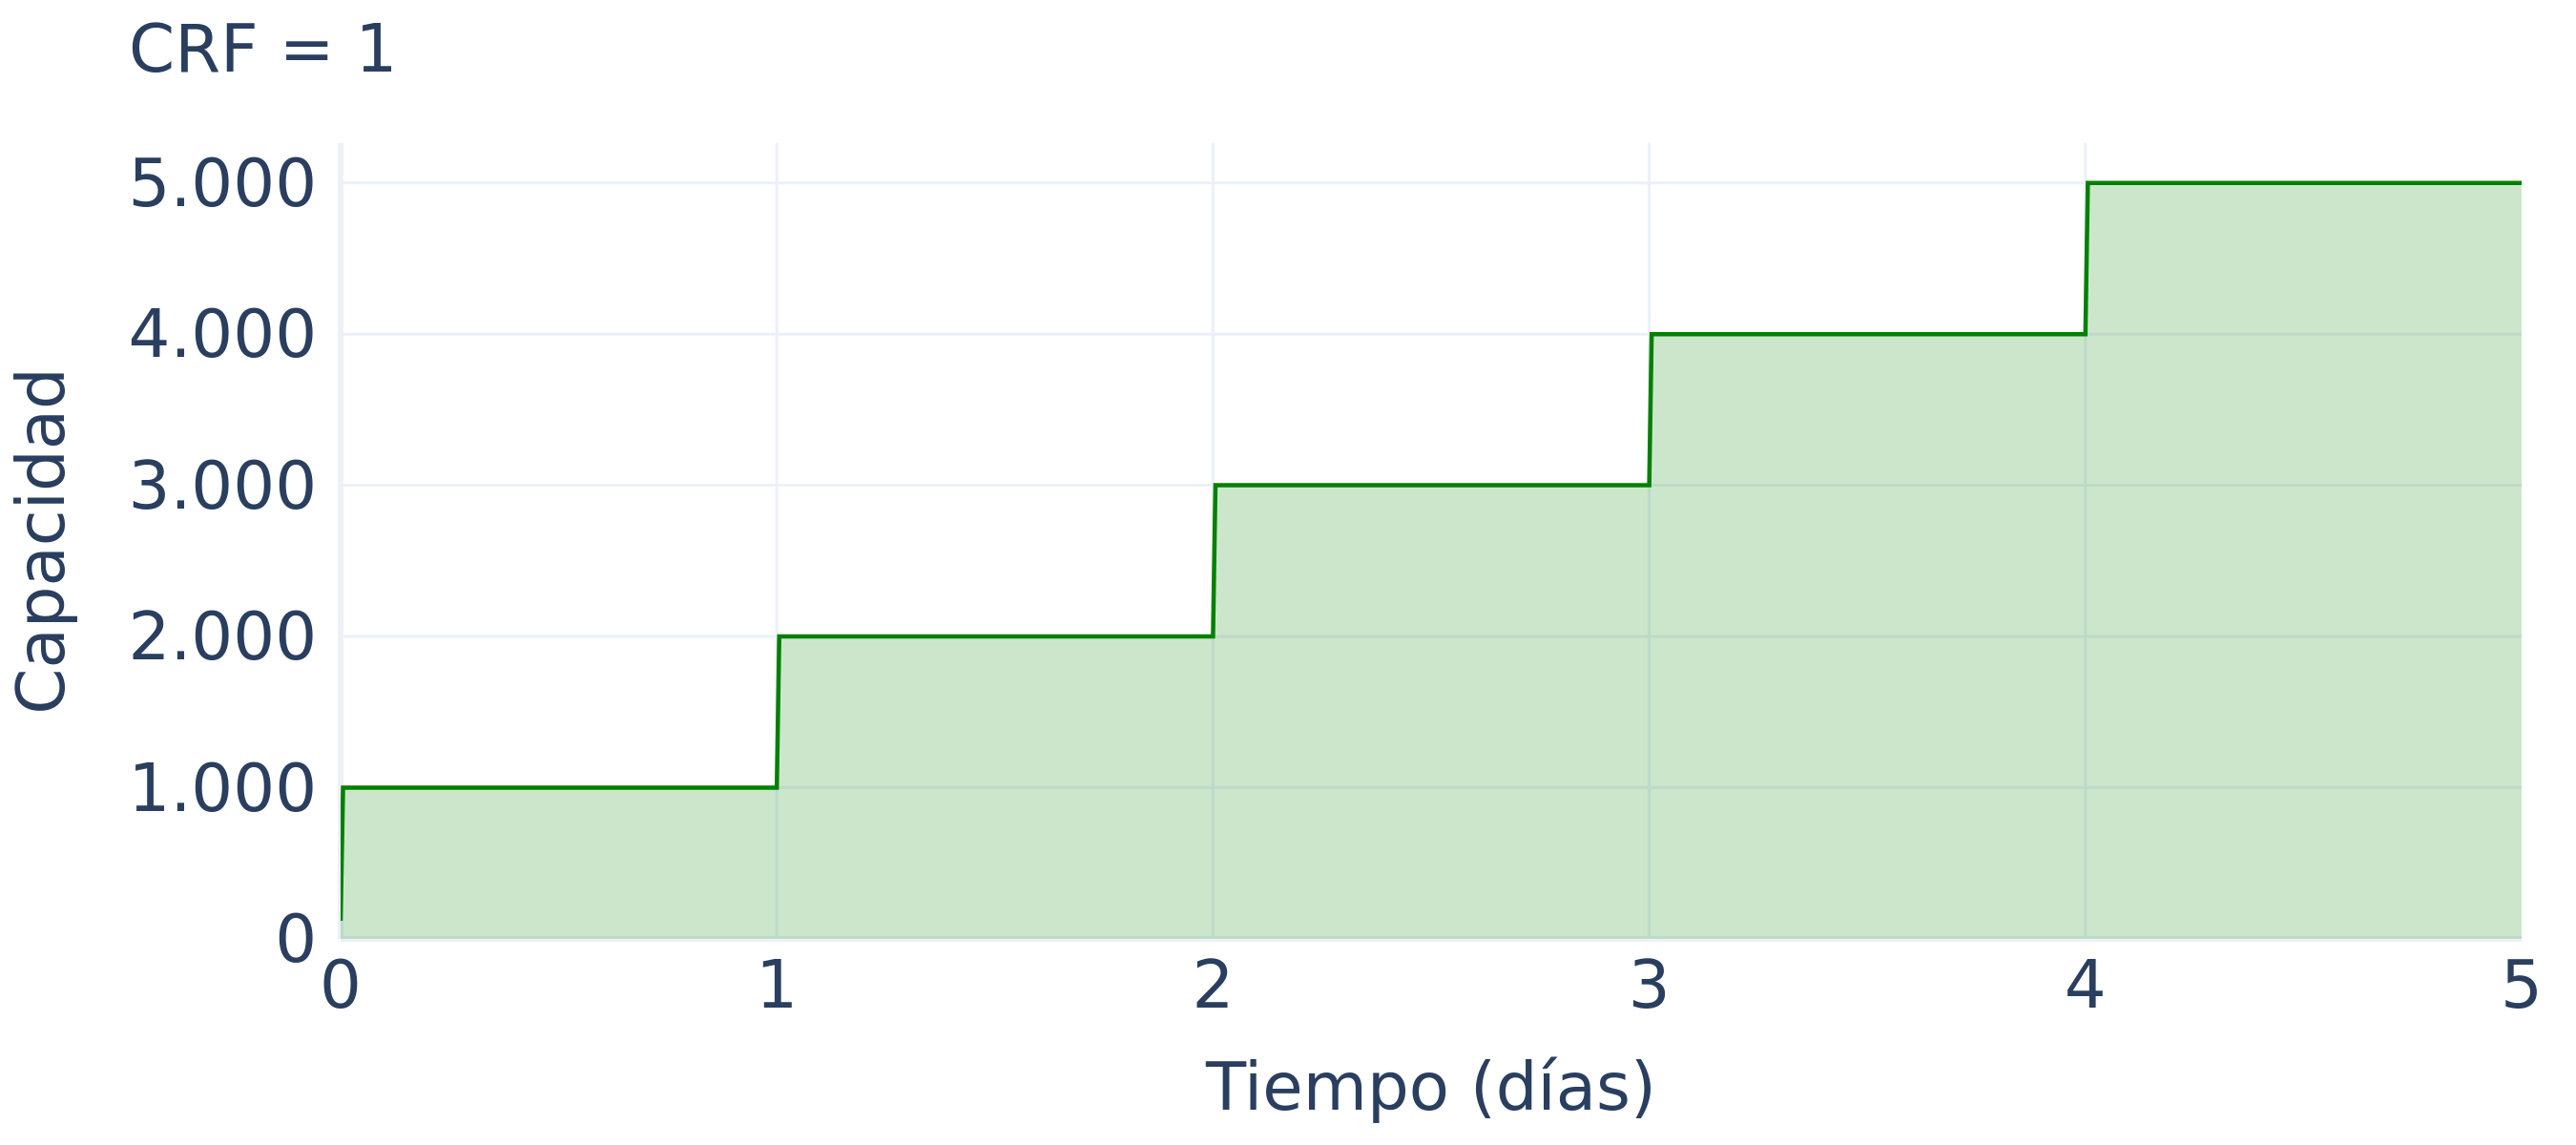
\includegraphics[width=0.72\textwidth]{fig/capacidad_mailersend_hobby_k1_peticiones_2026-10-25.png}
\caption[Curva de capacidad de MailerSend Hobby en peticiones]{Curva de capacidad de MailerSend Hobby con $k = 1$ sobre cinco días, pedida a PRIME4API \citep{prime4apirepo} en peticiones. Es la misma llamada que la gráfica (c) de la Figura~\ref{fig:capacidad}, con \texttt{capacity\_unit} en peticiones. La cuota diaria de 1.000 peticiones del plan sí entra, y la curva sube 1.000 cada medianoche UTC hasta los 5.000 de la cuota mensual el quinto día. Con $k = 1$ cada petición lleva un correo, así que la curva se lee también en correos. El tramo de \textit{rate} (120 peticiones por minuto durante ocho minutos) no se distingue a esta escala.}
\label{fig:limites:hobby-peticiones}
\end{figure}

El renderizador del motor oculta las curvas en peticiones.
Si se le pide la gráfica de MailerSend Hobby sin filtrar la unidad, devuelve cuatro figuras y las cuatro son de correos.
La curva en peticiones, la única que lleva la cuota diaria de Hobby, solo se dibuja con el parámetro \texttt{show\_derived\_requests}, cuyo valor por defecto es falso.
El \textit{endpoint} de datos, en cambio, devuelve las dos unidades sin que se le pida, así que la ausencia está solo en el dibujo.

La conversión que falta corresponde al motor.
La Datasheet de MailerSend declara los tres límites con su unidad y el factor $k$ que haría falta, que el motor usa en las otras dos conversiones.
MailerSend es la única de las ocho APIs que declara cuotas en dos unidades, y por eso el problema solo aparece en ella.
El defecto no cambia el plan más barato en ninguna de las tres recomendaciones de presupuesto del contraste, para 12.000, 25.000 y 40.000 correos.
Queda una pregunta que el catálogo no convierte en propuesta: una Datasheet con límites en dos unidades no declara en cuál mide el plan el proveedor, y quien la consulta elige la unidad al preguntar.

\subsection{Capacidad con un presupuesto menor que el precio del plan}

La operación \texttt{/capacity-at} calcula cuántos correos caben hasta una fecha con un presupuesto dado.
Con un presupuesto menor que el precio del plan, devuelve la cuota base más la primera ráfaga de la ventana siguiente.
En MailerSend Professional con 50 USD responde 50.120 correos y no marca el plan como no asequible, a diferencia de \texttt{/budget/recommendation}, que recomienda planes según el presupuesto y sí lo marca.
SendGrid Pro, que cuesta 89,95 USD al mes, responde 110.000 correos con el mismo presupuesto de 50 USD.

Brevo Professional cuesta 499 USD al mes, y con 50 USD el motor devuelve 151.000 correos con la categoría de caudal General y 152.000 con la Advanced.
Son los 150.000 de la cuota más lo que cabe en el primer segundo de la ventana siguiente, así que la categoría de caudal no cambia el volumen del mes.
En los tres casos el motor no amplía la cuota con sobrecoste, porque el presupuesto no cubre el precio del plan, pero devuelve igualmente la cuota base y no avisa de que el plan no es asequible.
Quien consulta \texttt{/capacity-at} con un presupuesto menor que el precio del plan tiene que cruzar la respuesta con \texttt{/budget/recommendation} para saber si puede pagar el plan.

El contraste cubre las ocho Datasheets del catálogo. Una API con cuotas en tres unidades o con un sobrecoste que exija aprobación previa podría sacar a la luz convenciones del motor que estas ocho no activan.

\section{Respuesta a la RQ3}
\label{sec:limites:respuesta}

La RQ3 pregunta cómo se relacionan los límites de uso y los \textit{rates} en las APIs de correo, y qué implicaciones tiene esa relación para el consumidor.

En seis de las ocho APIs (Postmark, Resend, SendGrid, MailerSend, Brevo y Mailgun) la cuota es la restricción activa, el límite que se alcanza primero y frena el envío (Sección~\ref{sec:limites:geometrica}).
En lo que el \textit{rate} admite durante la ventana cabe entre 103,7 veces la cuota (MailerSend Starter) y 129.600.000 veces (el plan Free de Postmark, cuyo \textit{rate} no está publicado y sale de la cabecera que devuelve la API).
La condición es que el \textit{rate} y la cuota tengan valor en la Datasheet, publicado o medido, y que la cuenta no esté en revisión, en pruebas ni restringida por reputación.
Con esa condición, quien contrate una de las seis puede dimensionar el volumen sin consultar el \textit{rate}.

El cociente $R \cdot W / Q$ baja a 2,59 en MailerSend Professional 2M, un volumen contratado que la Datasheet no recoge, y a 0,43 en Starter 1M con la cuenta en revisión, el único caso de las dos tablas con cociente calculable en que manda el \textit{rate}.
En Amazon SES y Mailchimp Transactional no se puede decir que mande la cuota.
Amazon SES no publica la cuota ni el caudal de producción, así que la relación no se puede calcular antes de sacar la cuenta del entorno de pruebas.
En Mailchimp Transactional la restricción activa es el caudal: la cuenta de prueba tiene una franquicia de 500 correos y un tope de 25 correos por hora, de modo que agotarla lleva 20 horas.

Las implicaciones para quien contrata salen de tres casos en que la cuota no basta para dimensionar el envío.
El primero es el estado de la cuenta, que condiciona la capacidad en seis de las ocho APIs sin que ninguna publique el umbral que dispara el cambio.
Solo MailerSend da una cifra para cada estado, 120 peticiones por minuto con la cuenta sana frente a 10 en revisión.

El segundo caso es la distancia entre el \textit{rate} publicado y el observado.
Solo coinciden en cuatro APIs, las que escriben a qué se aplica el valor.
Resend lo fija para cada equipo de la cuenta, MailerSend para cada estado de la cuenta, Brevo para cada \textit{endpoint} en su categoría General y Mailchimp Transactional para la cuenta de prueba.
En Mailgun, en cambio, no coinciden las 1.500 peticiones por segundo y por IP de sus preguntas frecuentes y el contador de la cabecera del envío, 80.000 peticiones por ventana de unos diez segundos.

Amazon SES y Mailchimp Transactional no emiten ninguna cabecera de caudal, y Mailgun solo la devuelve tras un envío aceptado.
Para comprobar antes de enviar cuánta capacidad queda hace falta un \textit{endpoint} que la informe, y solo la mitad del catálogo lo tiene.
Amazon SES, Mailchimp Transactional y MailerSend devuelven el límite, y Brevo solo el saldo de correos.

El tercer caso es el factor $k$, los destinatarios por petición, que pasa el \textit{rate} de peticiones a correos.
Solo vale si cada destinatario descuenta un correo de la cuota, y eso solo consta en Resend, SendGrid, Brevo y Amazon SES.
En Postmark, MailerSend, Mailgun y Mailchimp Transactional el paso de peticiones a correos es una suposición.

El contraste con PRIME4API de la Tabla~\ref{tab:a06-presupuesto}, que da el tiempo mínimo para enviar 100.000 correos con y sin presupuesto, añade dos implicaciones más.
La primera es que la Datasheet no dice cuál de los dos regímenes aplica el proveedor: en Postmark Basic, la respuesta es de 270 días si la cuota es un corte estricto y de 19 segundos si se paga el sobrecoste.
La segunda es que el motor lee como infinito el caudal que la Datasheet deja vacío: con ese bloque vacío, agotaba en 0 segundos los 10.000 correos de Postmark Basic, cuyo \textit{rate} el proveedor no publica.

En el borde de la cuota hay tres comportamientos, que recoge la Sección~\ref{sec:limites:catalogo} y no el contraste con el motor.
Amazon SES rechaza la llamada y descarta el mensaje, y SendGrid, MailerSend y Mailchimp Transactional detienen el envío donde no hay sobrecoste.
Brevo retiene en cola hasta 1.000 correos por encima de la cuota diaria y no entrega los que pasan de esa cifra, que es lo que modela la propuesta P-09 del Apartado~\ref{subsec:evolucion:p09}.

Esta respuesta descansa sobre una base estrecha.
El par formado por el \textit{rate} y la cuota solo tiene valor en la Datasheet de seis APIs.
En cuatro de ellas el proveedor publica el \textit{rate} del envío, y en Postmark y Mailgun sale de una cabecera medida: en Mailgun, 80.000 peticiones por una ventana de unos diez segundos, que la Tabla~\ref{tab:limites-rates-b} divide entre diez.
La cifra que Mailgun publica, 1.500 peticiones por segundo y por IP, tiene otro ámbito.
De los cuatro \textit{rates} publicados, el de SendGrid no se liga a ningún plan y el de Resend es el valor por defecto del equipo.
El de MailerSend solo vale para una cuenta aprobada, y la página de Brevo se contradice sobre qué planes incluyen cada una de sus tres categorías de caudal.

Los valores medidos tampoco describen el plan contratado: en MailerSend, Amazon SES y Mailchimp Transactional corresponden a cuentas sin aprobar o en pruebas, y en Postmark y Mailgun a una sola cuenta gratuita.
La relación entre cuota y \textit{rate} queda establecida en seis APIs, pero el margen exacto entre ambos depende de valores que los proveedores no fijan por escrito.

